% Research presentation. Compile from model-report/: latexmk -pdf presentation.tex
\documentclass[aspectratio=169,11pt]{beamer}

\usepackage{booktabs,amsmath,tikz}
\usetikzlibrary{arrows.meta,positioning}
\graphicspath{{figures/}{../figures/}}

\definecolor{navy}{HTML}{1F4E79}
\definecolor{headerblue}{HTML}{CDDEEF}
\definecolor{teal}{HTML}{2F6F6A}
\setbeamercolor{structure}{fg=navy}
\setbeamercolor{frametitle}{bg=headerblue,fg=navy}
\setbeamercolor{title}{fg=navy}
\setbeamercolor{itemize item}{fg=navy}
\setbeamertemplate{navigation symbols}{}
\setbeamertemplate{footline}{%
  \hspace{4mm}{\scriptsize\color{navy} amysteriousdataset}%
  \hfill{\scriptsize\color{navy}\insertframenumber\,/\,\inserttotalframenumber}%
  \hspace{4mm}\vspace{1.5mm}}
\setbeamerfont{frametitle}{size=\large,series=\bfseries}
\setbeamertemplate{itemize items}[circle]
\setlength{\leftmargini}{1.1em}

\newcommand{\md}[1]{\textbf{#1}}

\tikzset{
  box/.style={draw=navy, rounded corners=2pt, align=center,
              fill=navy!6, inner sep=3pt, font=\scriptsize},
  emphbox/.style={box, fill=navy!16},
  arr/.style={-{Stealth[length=1.8mm]}, semithick, navy}
}

\title{Predicting Toronto Home Sale Prices:\\ Two Valuation Scenarios}
\subtitle{SSU Data Dash 2026}
\author{Amy Dang Phuong, Maira Masroor, Shannon Tanoto, Yiwei Jiang}
\date{}

\begin{document}

\begin{frame}
\titlepage
\end{frame}

\begin{frame}{Two valuation scenarios}
\begin{columns}[c,onlytextwidth]
\begin{column}{0.48\textwidth}
\textbf{\color{navy} Off-market}\\[3pt]
No asking price. The level has to come from the home and from sales that have already closed.\\[4pt]
Target \quad \(\log Y\)\\[4pt]

\vspace{3pt}
\textbf{\color{navy} List-aware}\\[3pt]
The asking price \(L\) is known. The target is the gap around that ask.\\[4pt]
Target \quad \(\log(Y/L)\)\\[5pt]
{\small \(Y\) is the sold price. The dollar price is the ask times the predicted ratio.}
\end{column}
\begin{column}{0.50\textwidth}
\centering
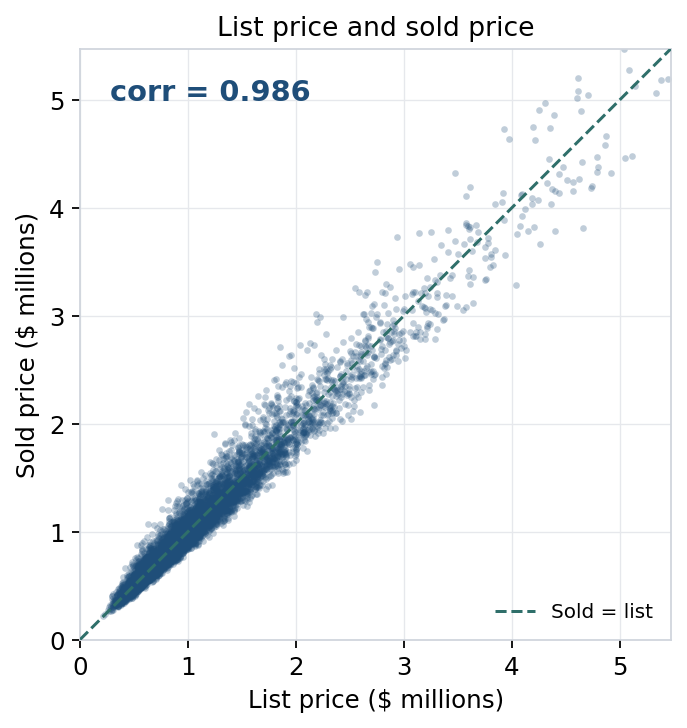
\includegraphics[width=0.94\linewidth]{pres_list_vs_sold.png}
\end{column}
\end{columns}
\end{frame}

\begin{frame}{Dataset overview and market dynamics}

{\small \(150{,}000\) synthetic Toronto sales, January 2021--May 2026. Attributes, location, listing text, dates, and prices. No external data. Full-book median sold/list ratio \(0.98\).}

\vspace{8pt}
\begin{columns}[c]
\begin{column}{0.50\textwidth}
\centering
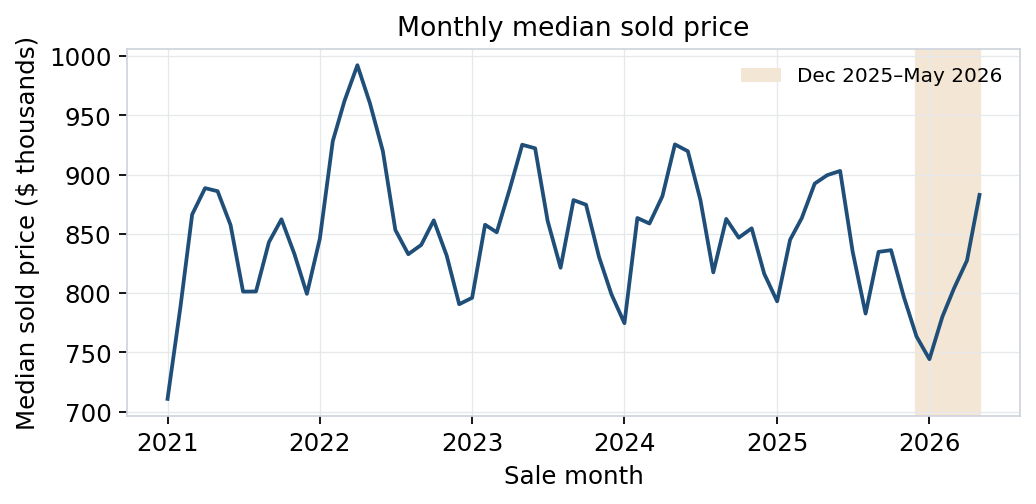
\includegraphics[width=\linewidth]{pres_median_price.png}
\end{column}
\begin{column}{0.50\textwidth}
\centering
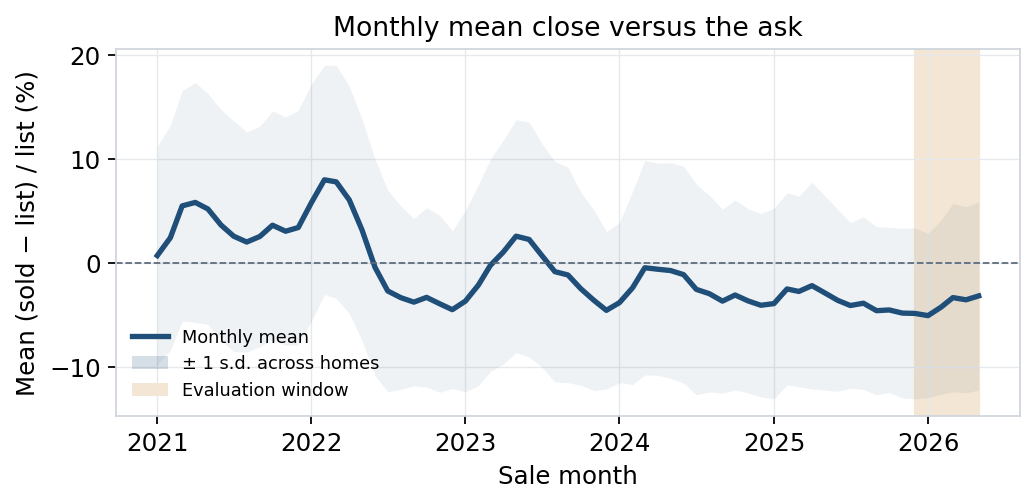
\includegraphics[width=\linewidth]{pres_close_vs_list.png}
\end{column}
\end{columns}

\vspace{2pt}
% {\scriptsize Beige band: the December 2025--May 2026 evaluation window. Blue band: \(\pm 1\) s.d.\ across homes in that month, not a confidence interval. The price level moves, and the gap between ask and close is not a fixed discount.}
\end{frame}

\begin{frame}{Data preparation and feature engineering}
\begin{columns}[c]
\begin{column}{0.48\textwidth}
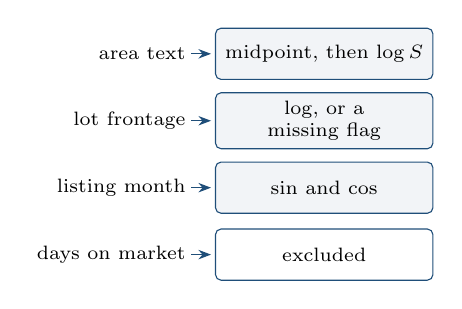
\begin{tikzpicture}[
  arr/.style={-{Stealth[length=1.6mm]}, navy},
  raw/.style={font=\scriptsize, anchor=east},
  xform/.style={box, text width=2.55cm, minimum height=6.5mm, font=\scriptsize, anchor=west}
]
\node[raw] (a) at (0,0) {area text};
\node[xform] at (0.25,0) {midpoint, then \(\log S\)};
\node[raw] (b) at (0,-0.85) {lot frontage};
\node[xform] at (0.25,-0.85) {log, or a missing flag};
\node[raw] (c) at (0,-1.7) {listing month};
\node[xform] at (0.25,-1.7) {\(\sin\) and \(\cos\)};
\node[raw] (d) at (0,-2.55) {days on market};
\node[xform, fill=white] at (0.25,-2.55) {excluded};
\draw[arr] (-0.05,0) -- (0.2,0);
\draw[arr] (-0.05,-0.85) -- (0.2,-0.85);
\draw[arr] (-0.05,-1.7) -- (0.2,-1.7);
\draw[arr] (-0.05,-2.55) -- (0.2,-2.55);
\end{tikzpicture}
\end{column}
\begin{column}{0.52\textwidth}
\centering
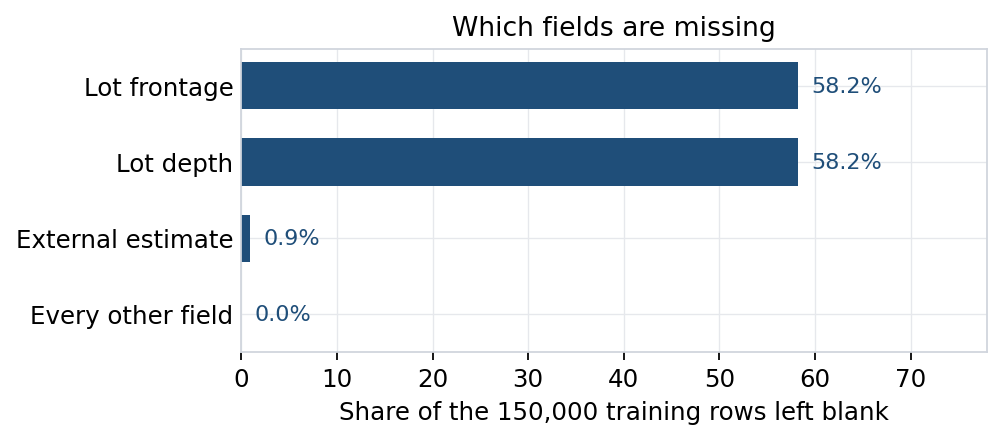
\includegraphics[width=\linewidth]{report_lot_missing.png}\\
{\scriptsize The lot blanks are the same rows. They are the condominiums.}
\end{column}
\end{columns}
\end{frame}

\begin{frame}{Off-market model development}
\[
A_i=S_i\, m_{c(i),t(i)}(\tau_i)
\]
{\small \(m\): median sold \$/sqft, same community and type, 12 months before listing. Fewer than 30 sales falls back to the type, then the city.}

\vspace{6pt}
\begin{tabular}{lr}
\toprule
Formulation & MdAPE \\
\midrule
Historical anchor & 15.60\% \\
LightGBM on the anchor residual & 7.54\% \\
Direct log-price LightGBM & 7.53\% \\
\bottomrule
\end{tabular}

\vspace{8pt}
{\small One fit through November 2025, scored on December 2025--May 2026. Not the walk-forward refit.}
\end{frame}

\begin{frame}{Off-market: historical sales and property information}
\begin{center}
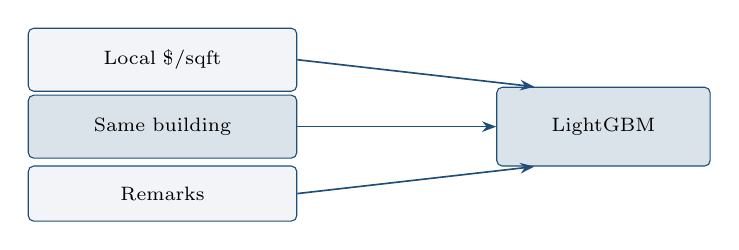
\begin{tikzpicture}
\node[box, text width=3.2cm, minimum height=8mm] (tape) at (0,0.85) {Local \$/sqft};
\node[emphbox, text width=3.2cm, minimum height=8mm] (bldg) at (0,0) {Same building};
\node[box, text width=3.2cm, minimum height=7mm] (rem) at (0,-0.85) {Remarks};
\node[emphbox, text width=2.5cm, minimum height=1cm] (tree) at (5.6,0) {LightGBM};
\draw[arr] (tape.east) -- (tree.150);
\draw[arr] (bldg.east) -- (tree.west);
\draw[arr] (rem.east) -- (tree.210);
\end{tikzpicture}
\end{center}

\vspace{1pt}
{\small Illustrative comparable. Not a fitted home.}

\vspace{2pt}
{\large
\begin{tabular}{ccccc}
\toprule
Earlier \$/sqft & Index then & Index now & Brought forward & Column \\
\midrule
\$640 & 100 & 108 & \$691 & \(\log(S\times 691)\) \\
\bottomrule
\end{tabular}}

\vspace{4pt}
{\scriptsize Index \(=\exp(I_{t,m})\), \(I\) a three-month median of earlier log \$/sqft. Coverage \(59.8\%\). Remarks are \(0.7\%\) of split gain.}
\end{frame}

\begin{frame}{Off-market architecture and calibration}
\[
\hat Y=\exp\bigl(F(x)\bigr)\,\exp(-\delta),
\qquad
\delta=\operatorname{median}_{j\in\mathrm{recent}}\bigl(\log\tilde Y_j-\log Y_j\bigr)
\]
{\small A positive \(\delta\) is recent overprediction. The price is scaled by \(\exp(-\delta)\).}
\begin{center}
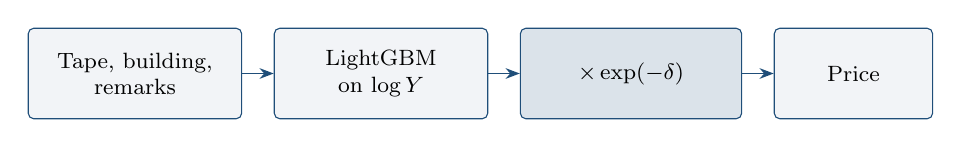
\begin{tikzpicture}[box/.append style={font=\footnotesize, minimum height=1.15cm}]
\node[box, text width=2.5cm] (a) {Tape, building,\\ remarks};
\node[box, text width=2.5cm, right=4mm of a] (b) {LightGBM\\ on \(\log Y\)};
\node[emphbox, text width=2.6cm, right=4mm of b] (c) {\(\times\exp(-\delta)\)};
\node[box, text width=1.8cm, right=4mm of c] (d) {Price};
\draw[arr] (a)--(b); \draw[arr] (b)--(c); \draw[arr] (c)--(d);
\end{tikzpicture}
\end{center}

\vspace{2pt}
{\small
\begin{tabular}{lrr}
\toprule
July--November 2025 screen & MdAPE & Median signed \\
\midrule
No correction & 8.31\% & \(+4.71\%\) \\
Full correction & \md{7.97\%} & \(+3.77\%\) \\
\bottomrule
\end{tabular}}

\vspace{3pt}
{\small The three months are before the origin, and the tree that measures \(\delta\) did not see them. This screen chose the weight. It is not the walk-forward claim.

\vspace{2pt}
LightGBM is the engine on both tracks: it splits on categories, missing values, and interactions among the home and the comps. On an earlier list-aware feature set it matched XGBoost and beat a random forest.}
\end{frame}

\begin{frame}{List-aware: the gap around the asking price}
\begin{columns}[c]
\begin{column}{0.46\textwidth}
The ask carries the level. A log-linear fit of \(\log Y\) on \(\log L\) and the attributes has elasticity \(0.894\) and \(R^2=0.966\).

\vspace{6pt}
\[
g_i=\log(Y_i/L_i),
\qquad
\hat Y_i=L_i\exp(\hat g_i).
\]

\vspace{4pt}
{\small Full-book median \(Y/L=0.98\), about \(2\%\) under the ask. The monthly mean of that gap is not flat.}
\end{column}
\begin{column}{0.52\textwidth}
\centering
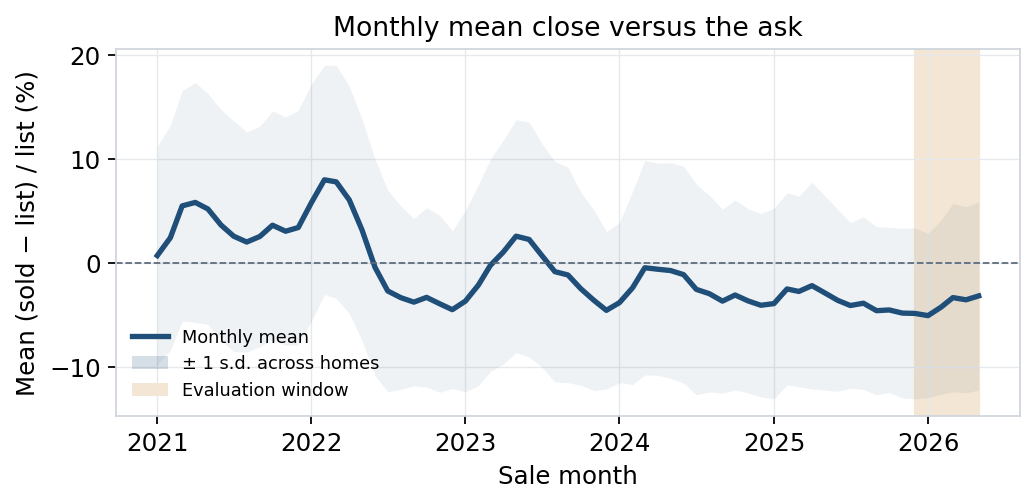
\includegraphics[width=\linewidth]{pres_close_vs_list.png}
\end{column}
\end{columns}
\end{frame}

\begin{frame}{Modeling temporal residuals with SARIMAX}
\[
\log Y_i=\beta_0+\beta_L\log L_i+z_i^\top\gamma+e_i
\qquad
(1-\phi L)(1-\Phi L^{12})\bar e_m=c+u_m
\]
\begin{center}
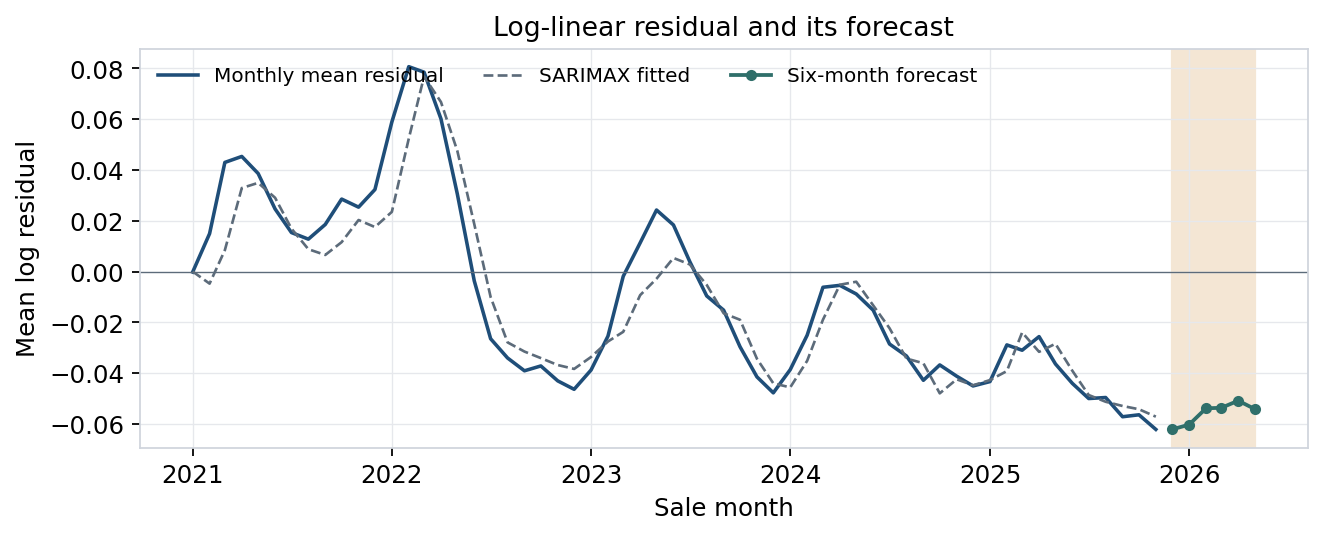
\includegraphics[width=0.74\textwidth]{pres_sarimax.png}
\end{center}
\vspace{-4pt}
{\scriptsize Fitted order \(\mathrm{SARIMAX}(1,0,0)\times(1,0,0,12)\). The product of the two autoregressions includes a lag-13 term.

\vspace{2pt}
\normalsize Putting that forecast on as a hard monthly shift, on the log-linear model alone, moves developmental MdAPE from \(7.13\%\) to \(4.78\%\) and the median signed error from \(+5.95\%\) to \(+0.25\%\). The tree does not apply that shift after the fact.}
\end{frame}

\begin{frame}{List-aware model specification}
\[
\hat Y=L\exp(\hat g)
\]
\begin{center}
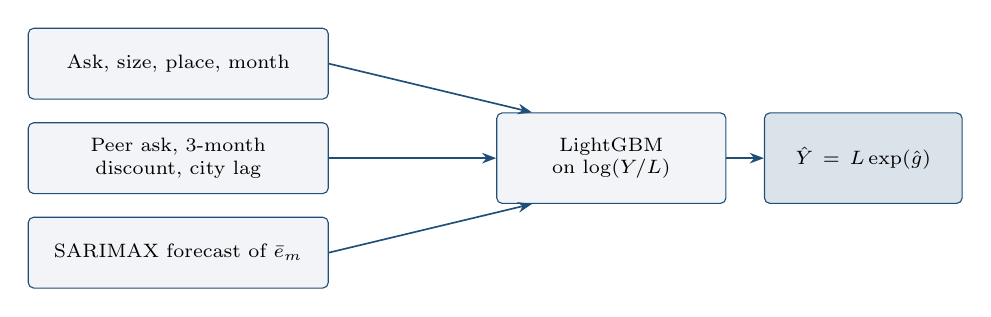
\begin{tikzpicture}
\node[box, text width=3.6cm, minimum height=9mm] (home) at (0,1.2)
  {Ask, size, place, month};
\node[box, text width=3.6cm, minimum height=9mm] (loc) at (0,0)
  {Peer ask, 3-month discount, city lag};
\node[box, text width=3.6cm, minimum height=9mm] (sx) at (0,-1.2)
  {SARIMAX forecast of \(\bar e_m\)};
\node[box, text width=2.7cm, minimum height=1.15cm] (tree) at (5.5,0)
  {LightGBM\\ on \(\log(Y/L)\)};
\node[emphbox, text width=2.3cm, minimum height=1.15cm] (price) at (8.7,0)
  {\(\hat Y=L\exp(\hat g)\)};
\draw[arr] (home.east) -- (tree.150);
\draw[arr] (loc.east) -- (tree.west);
\draw[arr] (sx.east) -- (tree.210);
\draw[arr] (tree) -- (price);
\end{tikzpicture}
\end{center}
\vspace{-1pt}
{\small The forecast is an input. The tree can use less of it on a home the monthly factor does not fit. A further shift after the tree had walk-forward signed error \(-1.75\%\) and was left off.}
\end{frame}

\begin{frame}{Walk-forward validation}
\begin{center}
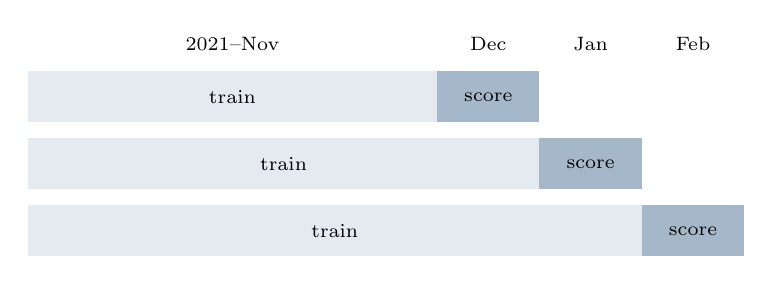
\begin{tikzpicture}[font=\scriptsize]
\node at (2.6,2.55) {2021--Nov};
\node at (5.85,2.55) {Dec};
\node at (7.15,2.55) {Jan};
\node at (8.45,2.55) {Feb};
\fill[navy!12] (0,1.55) rectangle (5.2,2.2);
\fill[navy!40] (5.2,1.55) rectangle (6.5,2.2);
\node at (2.6,1.87) {train};
\node at (5.85,1.87) {score};
\fill[navy!12] (0,0.7) rectangle (6.5,1.35);
\fill[navy!40] (6.5,0.7) rectangle (7.8,1.35);
\node at (3.25,1.02) {train};
\node at (7.15,1.02) {score};
\fill[navy!12] (0,-0.15) rectangle (7.8,0.5);
\fill[navy!40] (7.8,-0.15) rectangle (9.1,0.5);
\node at (3.9,0.17) {train};
\node at (8.45,0.17) {score};
\end{tikzpicture}
\end{center}

\vspace{1pt}
{\small March, April, and May repeat the step: the training bar grows by the month just scored. July--November 2025 was used only to choose the specification.}

\vspace{3pt}
{\small \(10{,}069\) sales. Tables, the SARIMAX, the ridge, the tree, and \(\delta\) are rebuilt on closes before the month being scored. A random split would put later closes into the comps.}
\end{frame}

\begin{frame}{Walk-forward performance}

{\small
\begin{tabular}{l c c r r}
\toprule
 & Baseline MdAPE & Model MdAPE & MAPE & Median signed \\
\midrule
Off-market & 15.33\% & \md{7.45\%} & 9.79\% & \(-0.37\%\) \\
List-aware & 7.26\% & \md{4.28\%} & 5.37\% & \(+0.90\%\) \\
\bottomrule
\end{tabular}}

\vspace{1pt}

\vspace{2pt}
\begin{columns}[c]
\begin{column}{0.50\textwidth}
\centering
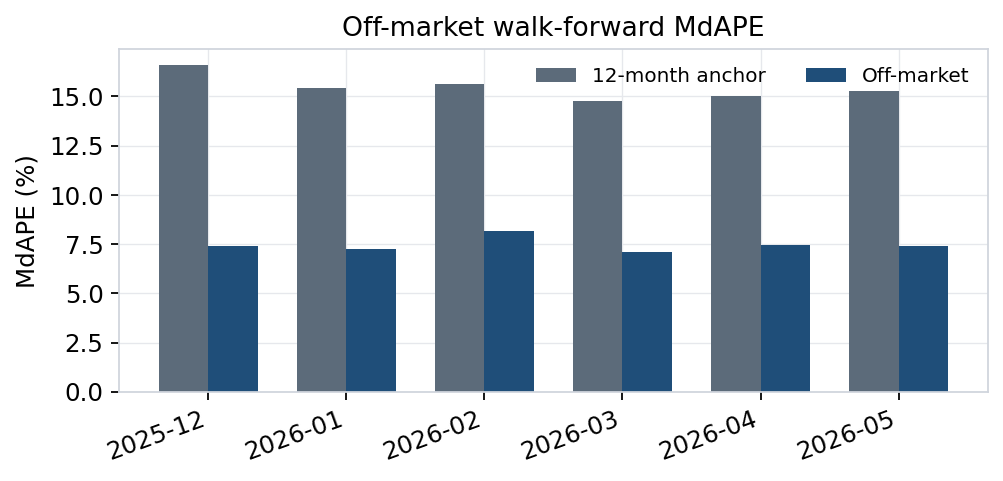
\includegraphics[width=\linewidth]{pres_om_mdape.png}
\end{column}
\begin{column}{0.50\textwidth}
\centering
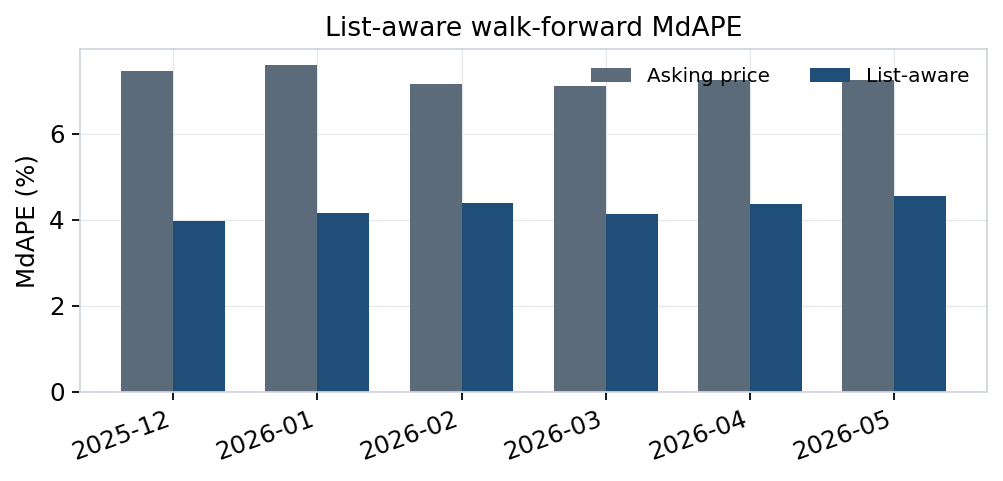
\includegraphics[width=\linewidth]{pres_la_mdape.png}
\end{column}
\end{columns}
\end{frame}

\begin{frame}{Feature importance}
\begin{columns}[c]
\begin{column}{0.50\textwidth}
\centering
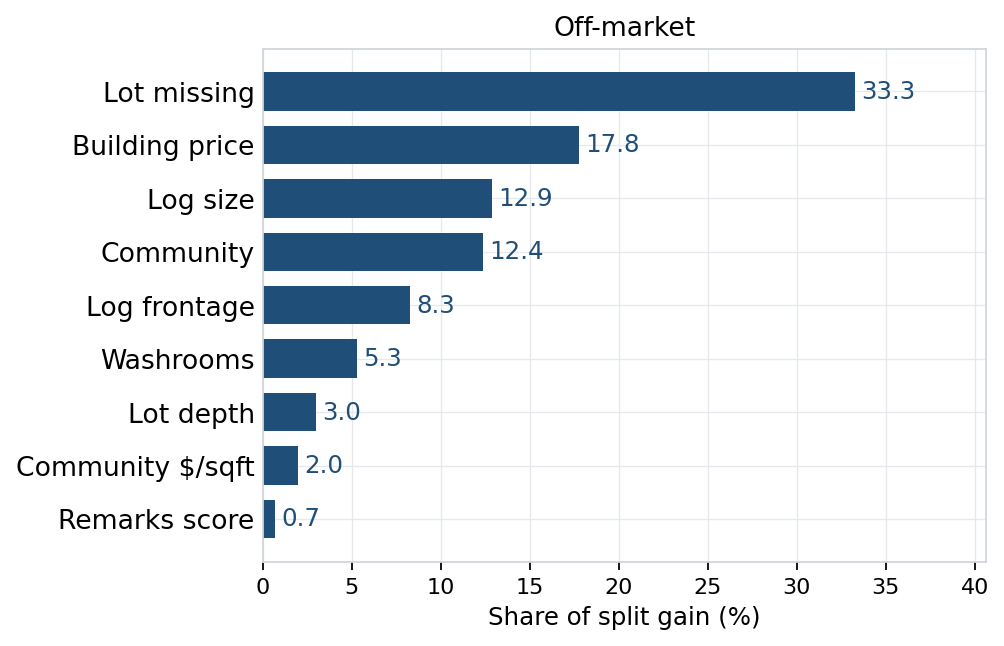
\includegraphics[width=\linewidth]{report_om_gain.png}
\end{column}
\begin{column}{0.50\textwidth}
\centering
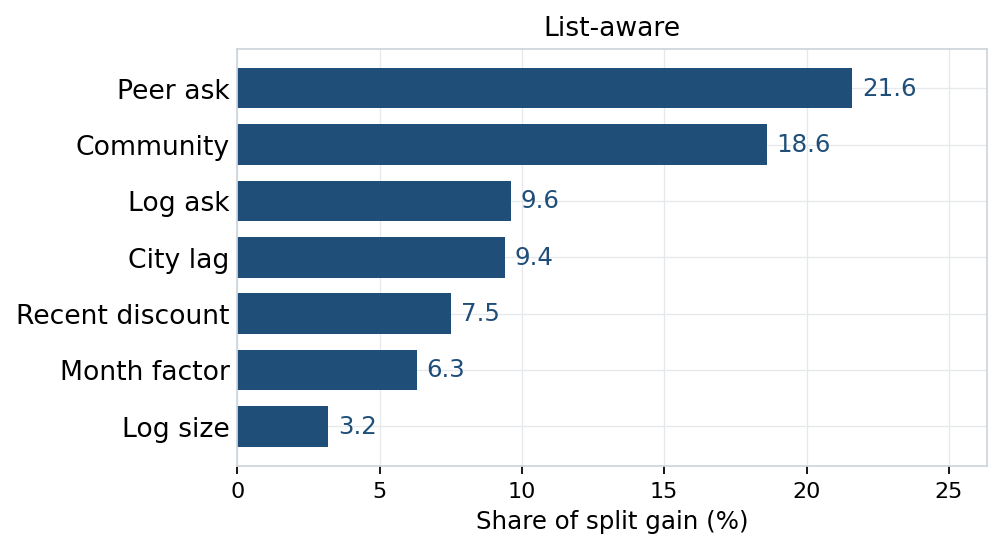
\includegraphics[width=\linewidth]{report_la_gain.png}
\end{column}
\end{columns}
\vspace{2pt}
% {\scriptsize Share of LightGBM split gain on the developmental fit. This describes where the fitted tree split. It is not a causal ranking.}
\end{frame}

\begin{frame}{Prediction errors by price}
\begin{columns}[c]
\begin{column}{0.50\textwidth}
\centering
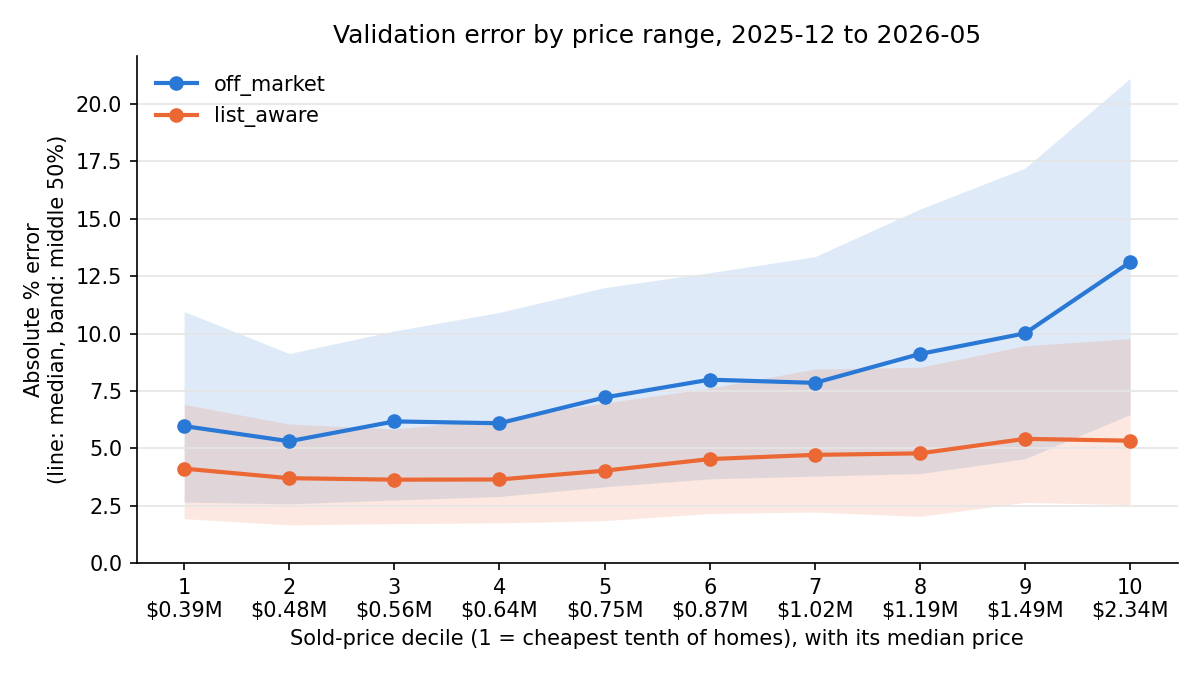
\includegraphics[width=\linewidth]{error_by_price_range.png}\\
{\scriptsize Absolute error: median, and the middle 50\%.\\[2pt]
Stale tape, May: MdAPE \(7.39\%\) to \(8.38\%\), signed \(+0.98\%\) to \(-5.29\%\).}
\end{column}
\begin{column}{0.50\textwidth}
\centering
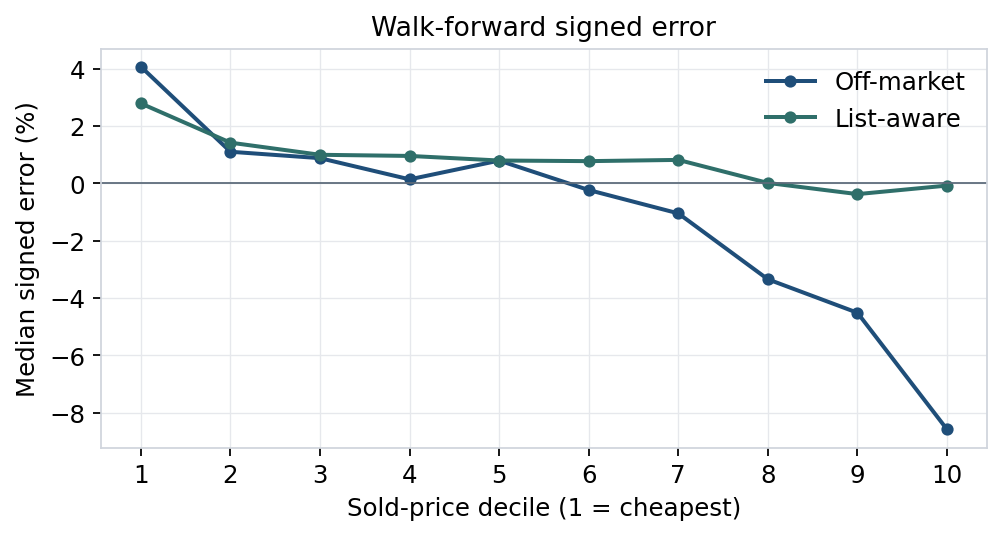
\includegraphics[width=\linewidth]{pres_signed_decile.png}\\
{\scriptsize Signed error. Same \(10{,}069\) sales and the same sold-price cuts. Positive means the prediction is high.}
\end{column}
\end{columns}
\end{frame}

\begin{frame}{Conclusions and limitations}
\begin{tabular}{@{}p{0.47\textwidth}@{\hspace{0.04\textwidth}}p{0.47\textwidth}@{}}
\textbf{\color{navy} Off-market} & \textbf{\color{navy} List-aware}\\[6pt]
{\Large 7.45\%} {\small MdAPE} & {\Large 4.28\%} {\small MdAPE}\\[3pt]
{\scriptsize 15.33\% baseline, a \(51\%\) reduction} &
{\scriptsize 7.26\% baseline, a \(41\%\) reduction}\\[6pt]
{\small Direct log-price prediction with historical comparable sales and recent-error calibration.} &
{\small Log closing ratio, with local market indicators and a SARIMAX feature.}
\end{tabular}

\vspace{6pt}
{\color{navy!25}\hrule height 0.4pt}
\vspace{6pt}

\textbf{Remaining limitations}

\vspace{5pt}
\begin{tabular}{@{}p{0.31\textwidth}@{\hspace{0.025\textwidth}}p{0.31\textwidth}@{\hspace{0.025\textwidth}}p{0.31\textwidth}@{}}
\textbf{\color{navy} Coverage} &
\textbf{\color{navy} Systematic bias} &
\textbf{\color{navy} Uncertainty}\\[5pt]
{\scriptsize\raggedright\hyphenpenalty=10000\exhyphenpenalty=10000 \(40\%\) lack an earlier same-building sale. \(46\%\) lack a recent local discount.\par} &
{\scriptsize\raggedright\hyphenpenalty=10000\exhyphenpenalty=10000 High-end underprediction off-market. Persistent positive bias, list-aware.\par} &
{\scriptsize\raggedright\hyphenpenalty=10000\exhyphenpenalty=10000 Synthetic data, point estimates, and dependence on recent historical sales.\par}
\end{tabular}

\vspace{6pt}
\begin{center}
\small Historical market information improves both valuation tasks, but accuracy depends on the availability and recency of comparable evidence.
\end{center}
\end{frame}

\end{document}
